\documentclass[10pt,spanish,aspectratio=1610]{beamer}
\usepackage[utf8]{inputenc}
\usepackage{amsmath}
\usepackage{graphicx}
\usepackage{amssymb}
\usepackage{multicol}
\usepackage[spanish]{babel}
\spanishdecimal{.}
\usepackage{subfig}
\usepackage{fancyhdr}
\usepackage{pstricks}
\usepackage{color}
\usepackage[ruled]{algorithm2e}
\usepackage{listings}
\usepackage{xcolor}
\usepackage{gensymb}
\usepackage{verbatim}

\definecolor{graywhite}{rgb}{0.9529,0.9607,0.9686}
\definecolor{bluegray}{rgb}{0.6823, 0.7411, 0.8}
\definecolor{darkred}{rgb}{0.7372, 0.2392, 0.2392}
\definecolor{bluedark}{rgb}{0.294, 0.4705, 0.6407}
\definecolor{darkgreen}{rgb}{0.1764, 0.5294, 0.0901}
\lstset{
  backgroundcolor=\color{graywhite},   % choose the background color; you must add \usepackage{color} or \usepackage{xcolor}; should come as last argument
  basicstyle=\footnotesize,        % the size of the fonts that are used for the code
  breakatwhitespace=false,         % sets if automatic breaks should only happen at whitespace
  breaklines=true,                 % sets automatic line breaking
  captionpos=b,                    % sets the caption-position to bottom
  commentstyle=\color{darkgreen},    % comment style
  keepspaces=true,                 % keeps spaces in text, useful for keeping indentation of code (possibly needs columns=flexible)
  keywordstyle=\color{darkred},       % keyword style
  language=Octave,                 % the language of the code
  morekeywords={*,...},            % if you want to add more keywords to the set
  numbers=left,                    % where to put the line-numbers; possible values are (none, left, right)
  numbersep=7pt,                   % how far the line-numbers are from the code
  numberstyle=\tiny\color{bluedark}, % the style that is used for the line-numbers
  showspaces=false,                % show spaces everywhere adding particular underscores; it overrides 'showstringspaces'
  showstringspaces=false,          % underline spaces within strings only
  showtabs=false,                  % show tabs within strings adding particular underscores
  stepnumber=1,                    % the step between two line-numbers. If it's 1, each line will be numbered
  stringstyle=\color{bluedark},     % string literal style
  frame=single,
  rulecolor=\color{bluegray},
  tabsize=2,                   % sets default tabsize to 2 spaces
  xleftmargin=1cm,
  xrightmargin=0.5cm,
  framexleftmargin=0.5cm,
  extendedchars=true,
  literate={á}{{\'a}}1 {é}{{\'e}}1 {í}{{\'i}}1 {ó}{{\'o}}1 {ú}{{\'u}}1 {Á}{{\'A}}1 {É}{{\'E}}1 {Í}{{\'I}}1 {Ó}{{\'O}}1 {Ú}{{\'U}}1,
}

\DeclareMathOperator{\atantwo}{atan2}
\setbeamercolor{block title}{fg=white,bg=blue!70!black}
\setbeamercolor{block body}{fg=black, bg=blue!10!white}
\setbeamertemplate{blocks}[rounded][shadow=false]
\setbeamercovered{transparent}
\beamertemplatenavigationsymbolsempty
\setbeamertemplate{frametitle}{
  \leavevmode
  \hbox{\begin{beamercolorbox}[wd=0.85\paperwidth,left]{frametitle}
    \usebeamerfont{frametitle}\insertframetitle
  \end{beamercolorbox}
%  \begin{beamercolorbox}[wd=0.25\paperwidth,center]{frametitle}
%    \usebeamerfont{frametitle}\hfill\hspace*{5ex}\footnotesize{\insertsubsection}
%  \end{beamercolorbox}
}}
\setbeamertemplate{footline}{
  \leavevmode%
  \hbox{%
    \begin{beamercolorbox}[colsep=-0.5pt,wd=.33\paperwidth,ht=3ex,dp=1.5ex,center]{author in head/foot}%
      \usebeamerfont{author in head/foot}\insertshortauthor~~ (\insertshortinstitute)
    \end{beamercolorbox}%
    \begin{beamercolorbox}[colsep=-0.5pt,wd=.34\paperwidth,ht=3ex,dp=1.5ex,center]{date in head/foot}%
      \usebeamerfont{author in head/foot}\insertshorttitle
    \end{beamercolorbox}%
    \begin{beamercolorbox}[colsep=-0.5pt,wd=.33\paperwidth,ht=3ex,dp=1.5ex,right]{author in head/foot}%
      \usebeamerfont{author in head/foot}\insertsection{}\hspace*{2em}\scriptsize{\insertframenumber{}}\hspace*{1ex}
    \end{beamercolorbox}
  }
}
\setbeamersize
{
    text margin left=0.25cm,
    text margin right=0.25cm
}

\begin{document}
\renewcommand{\tablename}{Tabla}
\renewcommand{\figurename}{Figura}

\title[Visión Computacional para Robótica]{Visión Computacional Aplicada a la Robótica}
\author[Marco Negrete]{Dr. Marco Negrete}
\institute[FI, UNAM]{Facultad de Ingeniería, UNAM}
\date[2023-2]{Semestre 2023-2}

\begin{frame}
\titlepage
\end{frame}

\begin{frame}\frametitle{Presentación del curso}
  \textbf{Objetivos:}
  \begin{itemize}
  \item Aprender los conceptos básicos de visión computacional enfocados a la solución de un problema particular: dotar de autonomía a un robot móvil
  \item Implementar dichos conceptos en un ambiente simulado
  \item Familiarizar al estudiante con diversas herramientas de software como ROS, Numpy y OpenCV
  \end{itemize}
\end{frame}


\begin{frame}\frametitle{Contenido}
  \begin{itemize}
  \item Introduction
  \item Procesamiento de Imágenes
  \item Modelo de una cámara
  \item Espacios de color
  \item Características (\textit{Features})
  \item Clasificación y reconocimiento
  \item Redes Neuronales
  \item Navegación visual 
  \end{itemize}
  \[\]
  \textbf{Bibliografía recomendada:}
  \begin{itemize}
  \item \url{https://drive.google.com/drive/folders/1gb7VQJG5eUkCvCginRHHGn5lez6VASBJ?usp=sharing}
  \item \url{https://drive.google.com/drive/folders/1Epl2b51xEJzCvzfugBD1i7xGdKYdJucy?usp=sharing}
  \end{itemize}
\end{frame}

\begin{frame}\frametitle{Forma de trabajo}
  \begin{itemize}
  \item Horario: Viernes de 10:00 a 13:00.\\
  \item Para la realización de ciertas tareas se utilizará el simulador Gazebo junto con la plataforma ROS Noetic. Este software corre en el sistema operativo Ubuntu 20.04. Las prácticas implicarán escribir código para lo cual se utilizará el repositorio\\
    \url{https://github.com/mnegretev/ComputerVisionForRobotics-2023-2}\\
    Si no se desea instalar el sistema operativo de forma nativa, en el repositorio hay una máquina virtual con todo el software ya instalado.
  \item Para el uso del material del curso, se recomienda manejar las siguientes herramientas:
    \begin{itemize}
    \item Sistema operativo Ubuntu
    \item Lenguajes Python y C++
    \item Software de control de versiones Git
    \end{itemize}
    Un conocimiento a nivel introductorio es suficiente.
  \item Los códigos de cada práctica se subirán al repositorio en la rama asignada para cada estudiante.
  \item Los reportes escritos se entregarán al inicio de la clase en la fecha asignada.
  \end{itemize}
  Habrá un grupo en Google Classroom para todos los avisos. 
\end{frame}

\begin{frame}\frametitle{Forma de evaluar}
  Rubros a evaluar:
  \begin{table}
  \begin{tabular}{lr}
    Prácticas & 50\%\\
    Examen    & 50\%\\
  \end{tabular}
  \end{table}
\end{frame}


\section{Introducción}

\begin{frame}\frametitle{¿Qué es la visión computacional?}
  \begin{itemize}
  \item \textbf{Visión Humana: } Se puede concebir como una tarea de procesamiento de información, que obtiene significado a partir de los estímulos percibidos por los ojos.
  \item \textbf{Visión Computacional: } Desarrollo de programas de computadora que puedan \textit{interpretar} imágenes. Es decir, realizar la visión humana por medios computacionales. 
  \end{itemize}
  \begin{figure}
    \centering
    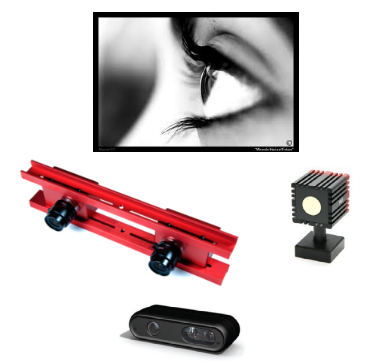
\includegraphics[width=0.5\textwidth]{Figures/VisionConcept.png}
  \end{figure}
\end{frame}

\begin{frame}\frametitle{Teoría de Marr}
“Visión es un proceso que produce, a partir de imágenes del mundo externo, una descripción que es útil para el observador y que está libre de información irrelevante.” (Marr, 1976).\\
El fenómeno de la visión lo podemos considerar como el producto de un sistema de procesamiento de información.\\

Marr propone los siguientes tres niveles de construcción de un sistema de procesamiento de información:\\
\begin{enumerate}
\item Teoría Computacional (¿Cuál es el problema por resolver?)
\item Representación y algoritmos (Estrategía usada para resolverlo)
\item Implementación (Realización física, software y hardware)
\end{enumerate}
Es decir, la visión computacional sería un proceso parecido a la visión humana, similar en los niveles computacionales y de algoritmos, pero implementado de forma diferente: en hardware de procesamiento con sensores de visión. 
\end{frame}

\begin{frame}\frametitle{Visión Computacional}
  Por lo tanto, la tarea de la Visión por computadora es la construcción de descriptores de la escena con base en características relevantes contenidas en una imagen:
  \begin{columns}
    \begin{column}{0.5\textwidth}
\begin{figure}
    \centering
    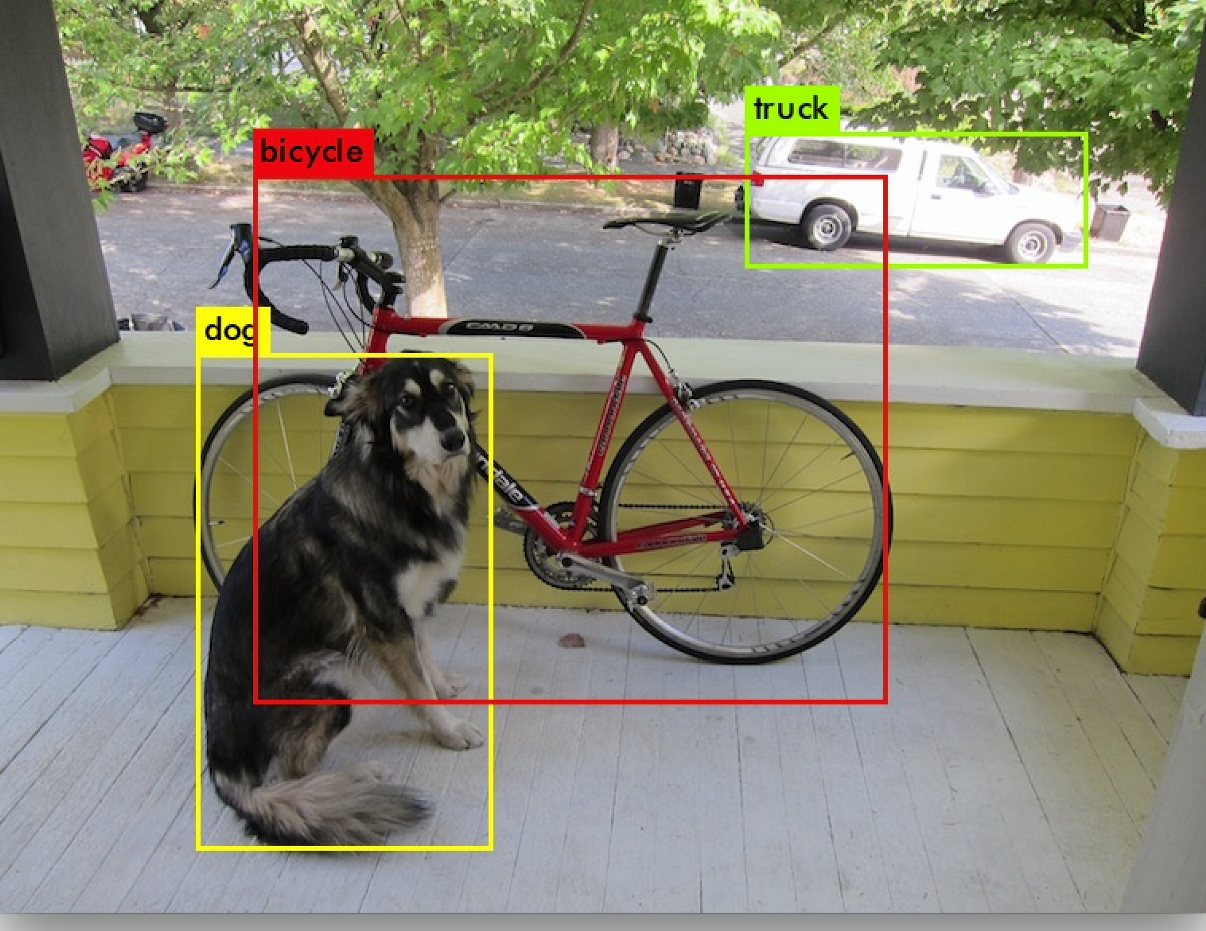
\includegraphics[width=0.8\textwidth]{Figures/Yolo.png}
\end{figure}
    \end{column}
    \begin{column}{0.5\textwidth}
\begin{itemize}
\item Objetos
\item Formas de Superficies
\item Colores
\item Texturas
\item Movimientos
\item Iluminación
\item Reflejos
\end{itemize}
    \end{column}
    \end{columns}
\end{frame}

\begin{frame}\frametitle{Vision Computacional vs Proc de Imágenes}
\begin{enumerate}
\item Procesamiento de imagenes: Es cualquier forma de procesamiento de señales donde la entrada es una imagen, la salida puede ser otra imagen o un conjunto de características o parámetros relacionados con la misma.
\item Visión Computacional: Estudio y aplicación de métodos que permiten a las computadoras “entender” el contenido de una imagen.
\item Visión Máquina: Es la aplicación de la visión por computadora en la industria y procesos de manufactura.
\end{enumerate}

\end{frame}

\begin{frame}\frametitle{Aplicaciones}
  Tareas que se pueden hacer con visión computacional (con aplicaciones a la robótica):
  \begin{itemize}
  \item OCR (Optical Character Recognition)
  \item Detección e identificación de rostros
  \item Reconocimiento de objetos
  \item Percepción para vehículos sin conductor
  \item Reconocimiento de gestos
  \end{itemize}
  Otras aplicaciones:
  \begin{itemize}
  \item Vigilancia
  \item Imagenología médica
  \item Consultas a bases de datos de imágenes.
  \item Percepción remota
  \end{itemize}
\end{frame}


\begin{frame}\frametitle{Esquema de Visión}
  \begin{figure}
    \centering
    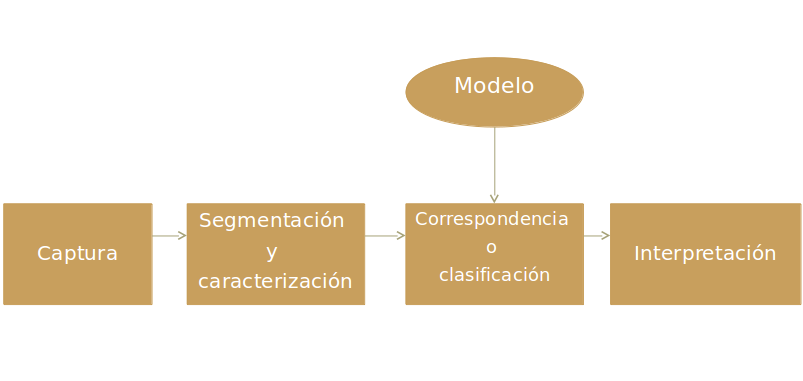
\includegraphics[width=1.0\textwidth]{Figures/VisionGeneralProcess.png}
  \end{figure}
\end{frame}


\begin{frame}\frametitle{Dificultades}

  El entorno real tiene una gran cantidad de variaciones en las imágenes de entrada.
  \begin{columns}
    \begin{column}{0.5\textwidth}
\begin{figure} %this figure will be at the right
    \centering
    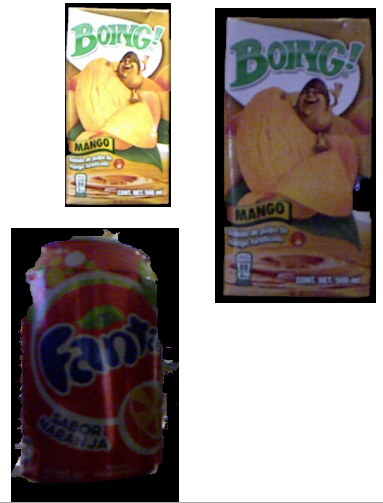
\includegraphics[width=0.5\textwidth]{Figures/VisionDificulties.png}
\end{figure}
    \end{column}
    \begin{column}{0.5\textwidth}
\begin{enumerate}
\item Iluminación
\item Orientación
\item Oclusión
\item Escala
\item Ruido
\item Desenfoque
\end{enumerate}
    \end{column}
  \end{columns}
\end{frame}

\begin{frame}\frametitle{Hardware y Software}
La computación con imágenes tiene mas de 30 años, sin embargo, en los últimos años, se ha incrementado considerablemente su desarrollo debido a:
\begin{enumerate}
\item Decremento en los precios 
\item Memoria con gran capacidad
\item Procesadores de propósito general de alta velocidad.
\item Existen scanners o camaras digitales que pueden ser utilizados para procesar imágenes propias.
\item Existen bibliotecas de software que contienen subrutinas de procesamiento de imágenes (opencv).
\end{enumerate}
\end{frame}



\section{OpenCV}

\begin{frame}\frametitle{OpenCV}
  \begin{columns}
    \begin{column}{0.5\textwidth}
      \begin{figure}
        \centering
        
\includegraphics[width=0.6\textwidth]{Figures/OpenCVLogo.png}
      \end{figure}
    \end{column}
    \begin{column}{0.5\textwidth}
      OpenCV es una biblioteca libre de visión artificial, originalmente desarrollada por Intel.
      
      Programación en código  Python, C y C++
      
      Existen versiones para GNU/Linux, Mac OS X y Windows
    \end{column}
    \end{columns}
    \end{frame}

\begin{frame}\frametitle{OpenCV}
\begin{figure}[h!]
        \centering
        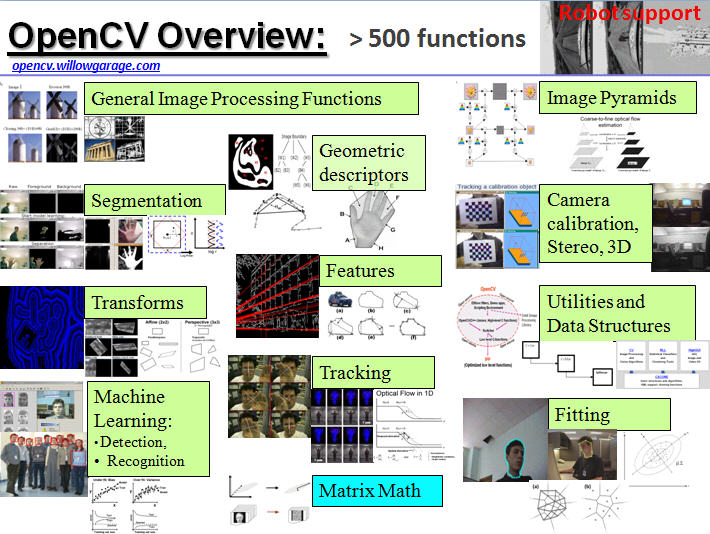
\includegraphics[width=0.75\textwidth]{Figures/OpenCVOverview.png}
\end{figure}
\end{frame}

\begin{frame}\frametitle{Funciones básicas}
  En Python, OpenCV está basado en la biblioteca Numpy por lo que muchas operaciones con imágenes corresponden a operaciones de Numpy sobre matrices.
  Algunas funciones que se usarán frecuentemente a lo largo del curso son:
  \begin{columns}
    \begin{column}{0.5\textwidth}
      \begin{itemize}
      \item \texttt{numpy.zeros}
      \item \texttt{enumpy.ones}
      \item \texttt{cv2.imread}
      \item \texttt{cv2.bitwise\_and}
      \item \texttt{cv2.bitwise\_or}
      \item \texttt{cv2.bitwise\_not}
      \item \texttt{cv2.bitwise\_xor}
      \end{itemize}
    \end{column}
    \begin{column}{0.5\textwidth}
      \begin{itemize}
      \item \texttt{cv2.inRange}
      \item \texttt{cv2.merge}
      \item \texttt{cv2.split}
      \item \texttt{cv2.imshow}
      \item \texttt{cv2.VideoCapture}
      \item \texttt{cv2.mean}
      \end{itemize}
    \end{column}
  \end{columns}
\end{frame}

\begin{frame}[containsverbatim]\frametitle{Ejercicio 1 - Lectura de imágenes y manejo de matrices}
  Escriba el siguiente código en un editor de texto:
  \lstinputlisting[language=Python]{Codes/Exercise01.py}
  Descargue la imagen \texttt{baboon.jpg} en la misma carpeta que el código. Abra una terminal y ejecute el código con el comando:
\begin{verbatim}
  python3 Exercise01.py
\end{verbatim}
  Modifique manualmente el tamaño de la imagen y modifique el código para que funcione con la imagen modificada. 
\end{frame}

\begin{frame}\frametitle{Operaciones lógicas}
  \begin{itemize}
  \item Las operaciones lógicas se usan generalmente para implementar \textit{máscaras}
  \item Puesto que son operaciones bit a bit, las imágenes a operar deben ser del mimo tamaño y tipo (mismo número de canales y mismo tipo de dato)
  \item Las máscaras suelen provenir de operaciones que dan como resultado imágenes binarias, como operaciones de comparación, umbralización o detección de bordes. 
  \end{itemize}
\end{frame}

\begin{frame}[containsverbatim]\frametitle{Ejercicio 2 - Operaciones lógicas bit a bit}
  Escriba el siguiente código en un editor de texto:
  \lstinputlisting[language=Python]{Codes/Exercise02.py}
  Ejecute el código y observe lo que hace cada operación.
\end{frame}

\begin{frame}[containsverbatim]\frametitle{Ejercicio 3 - Controles gráficos}
  \begin{itemize}
  \item OpenCV provee controles de interfaz gráfica de usuario que son útiles para la depuración de programas.
  \item Las barras de seguimiento (\textit{trackbars}) sirven para fijar valores en un intervalo y disparan una función \textit{callback} cuando hay un cambio en el valor.
  \item También provee \textit{callbacks} para el manejo de eventos del mouse (clicks derecho e izquierdo, movimiento del puntero, etc.)
  \end{itemize}
  Descargue el archivo \texttt{Exercise03.py}, ejecútelo y observe el comportamiento de la barra de seguimiento y de los clicks derecho e izquierdo. Consulte la documentación en línea y modifique el código para que se dibujen rectángulos con dimensiones dadas por dos clicks. 
\end{frame}

\begin{frame}\frametitle{Manejo de video}
  \begin{itemize}
  \item OpenCV provee la función \texttt{VideoCapture} para abrir fácilmente una cámara de video
  \item El video se entrega como una secuencia de imágenes por lo que un programa que maneje video debe contener un cilo \textit{while}
  \item La resolución más común es la de VGA de 640x480 aunque se pueden usar otras resoluciones dependiendo de las capacidades de cada cámara
  \item El número de cuadros por segundo (\textit{fps}) suele ser de 30, aunque puede ser de 60 o más, dependiendo de las capacidades de la cámara
  \item Si hay más de una cámara conectada, OpenCV las enumera con índices $i=0,1,2,3,\dots$ y se puede elegir qué cámara abrir usando dicho índice
  \item La misma funcion \texttt{VideoCapture} se puede usar para abrir videos en distintos formatos
  \end{itemize}
\end{frame}

\begin{frame}[containsverbatim]\frametitle{Ejercicio 4 - Manejo de vídeo}
  Escriba el siguiente código en un editor de texto:
  \lstinputlisting[language=Python]{Codes/Exercise04.py}
  El código anterior sólo abre una cámara y despliega la imagen en una ventana. Modifique el código para que realice lo siguiente:
  \begin{itemize}
  \item Cree una imagen en blanco y negro de dimensiones apropiadas similar a la del ejercicio 2
  \item Realice una o más operaciones lógicas entre el video y la imagen en blanco y negro
  \item Despliegue el resultado en una ventana
  \end{itemize}
\end{frame}

\section[Proc Imágenes]{Procesamiento de Imágenes}
\begin{frame}\frametitle{Imágenes como funciones}
  \begin{itemize}
  \item Una imagen (en escala de grises) es una función $I(x,y)$ donde $x,y$ son variables discretas en coordenadas de imagen y la función $I$ es intensidad luminosa.
    \item Las imágenes también pueden considerarse como arreglos bidimensionales de números entre un mínimo y un máximo (usualmente 0-255).
    \item Aunque formalmente una imagen es un mapeo $f:\mathbb{R}^2\rightarrow \mathbb{R}$, en la práctica, tanto $x,y$ como $I$ son varialbes discretas con valores entre un mínimo y un máximo.
    \item Las imágenes de color son funciones vectoriales $f:\mathbb{R}^2\rightarrow \mathbb{R}^3$ donde cada componente de la función se llama canal.
%  \[I(x,y) = \left[\begin{tabular}{c}$r(x,y)$\\$g(x,y)$\\$b(x,y)$\end{tabular}\right]\]
  \end{itemize}
  \begin{figure}
    \centering
    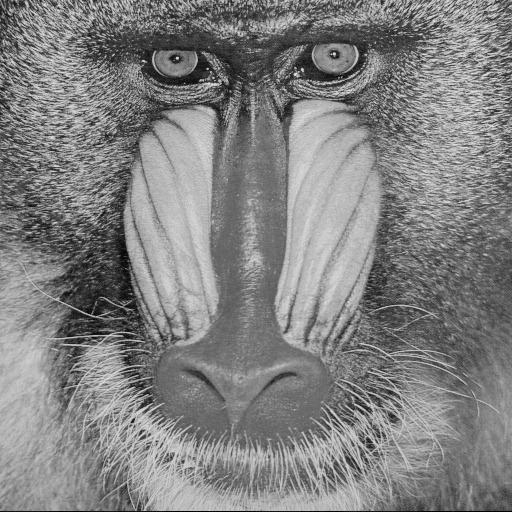
\includegraphics[width=0.3\textwidth]{Figures/baboon_grayscale.jpg}
    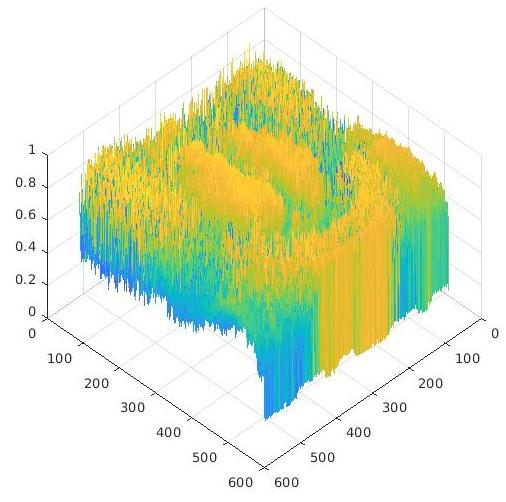
\includegraphics[width=0.35\textwidth]{Figures/BaboonPlot.jpg}
  \end{figure}
\end{frame}

\begin{frame}\frametitle{Operaciones básicas}
  Las operaciones básicas con una imagen son las mismas que con una señal cualquiera:
  \begin{itemize}
  \item Desfase
  \item Escalamiento
  \item Inversión en $x,y$
  \item Suma y Resta 
  \item Multiplicación
  \end{itemize}
  Ver ejercicios en Python.
\end{frame}

\begin{frame}\frametitle{Tipos de ruido}
  El ruido es una señal aleatoria $\eta(x,y)$, es decir, no sabemos cuánto vale para un punto determinado $(x,y)$ pero sí podemos caracterizarla.
  \[I_n(x,y) = I(x,y) + \eta(x,y)\]
  Existen varios tipos de ruido:
  \begin{itemize}
  \item Sal y pimienta: aleatoriamente aparecen puntos ya sea blancos o negros
  \item Ruido de impulso: aleatoriamente aparecen puntos blancos
  \item Ruido gausiano: $\eta(x,y)$ se distribuye 
  \end{itemize}
  Ver ejercicios en Python
\end{frame}

\begin{frame}\frametitle{SLID}
  Un sistema $S$ es un mapeo del conjunto de señales al conjunto de señales, es decir, es algo donde entra una señal $I(x,y)$ y sale otra señal $O(x,y)$:
  \[O(x,y) = S[I(x,y)]\]
  Los sistemas lineales invariantes ante el desfase son sistemas en los que se cumplen las siguientes propiedades:
  \begin{itemize}
  \item \textbf{Aditividad y homogeneidad:}
    \[S[\alpha I_1(x,y) + \beta I_2(x,y)] = \alpha S[I_1(x,y)] + \beta S[I_2(x,y)]\]
  \item \textbf{Invarianza ante el desfase:}
    \[\textrm{Si} \qquad S[I(x,y)] = O(x,y) \qquad\textrm{entonces:}\]
    \[S[I(x-i, y-j)] = O(x-i, y-j) \qquad \forall i,j \in \mathbb{Z}\]
  \end{itemize}
  Los SLID se pueden caracterizar de varias formas:
  \begin{itemize}
  \item Ecuaciones en diferencias
  \item Funciones de transferencia
  \item Respuesta al impulso
  \end{itemize}
\end{frame}

\begin{frame}\frametitle{Convolución}
  Si se conoce la respuesta al impulso $H(x,y)$ de un sistema SLID, se puede obtener la salida $O(x,y)$ ante cualquier entrada $I(x,y)$, mediante la convolución, definida como:
  \[O(x,y) = I(x,y)*H(x,y) = \sum_{i=-\infty}^\infty \sum_{j=-\infty}^\infty I(i,j)H(x-i, y-j)\]
  Ejemplos:
  \[\left[\begin{tabular}{cccc}
      3 & 1 & 4 & 1\\
      5 & 9 & 2 & 6\\
      5 & 3 & 5 & 8\\
      9 & 7 & 9 &3
    \end{tabular}\right]* [1\quad -1] =
  \left[\begin{tabular}{ccccc}
      3 & -2 & 3 & -3 & -1\\
      5 & 4 & -7 & 4 & -6\\
      5 & -2 & 2 & 3 & -8\\
      9 & -2 & 2 & -6 & -3
    \end{tabular}\right]\]

  \[\left[\begin{tabular}{cccc}
      3 & 1 & 4 & 1\\
      5 & 9 & 2 & 6\\
      5 & 3 & 5 & 8\\
      9 & 7 & 9 &3
    \end{tabular}\right]* \left[\begin{tabular}{c}1 \\ -1\end{tabular}\right] =
  \left[\begin{tabular}{cccc}
      3 & 1 & 4 & 1\\
      2 & 8 & -2 & 5\\
      0 & -6 & 3 & 2\\
      4 & 4 & 4 & -5\\
      -9 & -7 & -9 & -3
    \end{tabular}\right]\]
\end{frame}

\begin{frame}\frametitle{Manejo de bordes}
  En el ejemplo anterior, supusimos que fuera de la matriz, todos los elementos son cero. Sin embargo existen otras formas de manejar los borde:
  \begin{itemize}
  \item Recortar: suponer que fuera de la matriz los valores son cero. En el caso de una imagen, suponemos pixeles negros fuera de la imagen.
  \item Wrap around: suponer que la imagen es periódica.
  \item Borde repetido: suponer que los valores de los bordes se mantienen iguales fuera de la imagen.
  \item Reflexión: fuera de los bordes se tiene una imagen en espejo.
  \end{itemize}
\end{frame}

\begin{frame}\frametitle{Propiedades de la convolución}
  \begin{itemize}
  \item Es conmutativa: $H*I = I*H$
  \item Es asociativa: $H*I_1*I_2$ = $H*(I_1*I_2)$ = $(H*I_1)*I_2$
  \item Es distributiva: $H*(I_1 + I_2) = H*I_1 + H*I_2$
  \item Es lineal: $H*(\alpha I_1 + \beta I_2) = \alpha H*I_1 + \beta H*I_2$
  \end{itemize}
  En el caso de secuencias finitas bidimensionales:
  \begin{itemize}
  \item Si $I\in\mathbb{R}^{r_1\times c_1}$ y $H\in\mathbb{R}^{r_2\times c_2}$, entonces $(I*H) \in \mathbb{R}^{(r_1+r_2-1)\times (c_1 + c_2 - 1)}$
  \item Si $I\in\mathbb{R}^{r_1\times c_1}$ y $H\in\mathbb{R}^{r_2\times c_2}$, la complejidad de la convolución es del orden de $r_1 r_2 c_1 c_2$
  \end{itemize}
\end{frame}

\begin{frame}\frametitle{Conexión de sistemas SLID}
  Dos o más SLID se pueden conectar de dos formas distintas:
  \begin{itemize}
  \item Conexión en paralelo:
    \begin{figure}
      \centering
      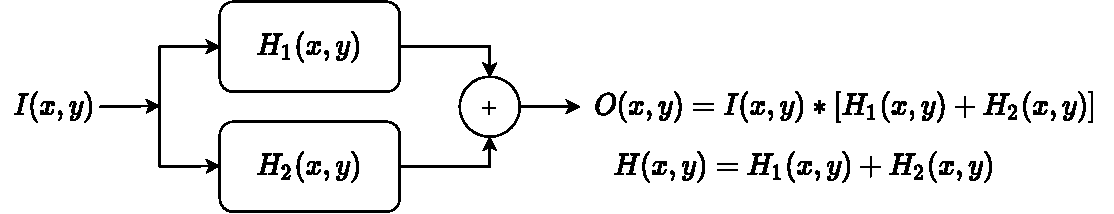
\includegraphics[scale=0.7]{Figures/Parallel.pdf}
    \end{figure}
  \item Conexión en cascada:
    \begin{figure}
      \centering
      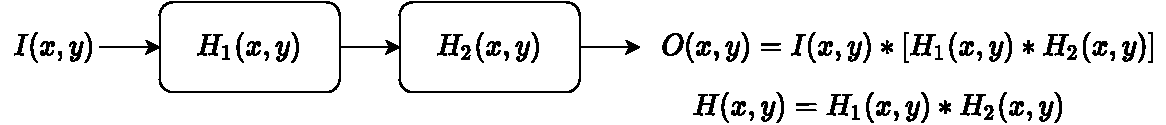
\includegraphics[scale=0.7]{Figures/Cascade.pdf}
    \end{figure}
  \end{itemize}
\end{frame}

\begin{frame}\frametitle{Gradiente}
  El gradiente de una imagen está definido como:
  \[\nabla I = \left[\frac{\partial I}{\partial x}, \frac{\partial I}{\partial y}\right]\]
  Las derivadas parciales se puede aproximar mediante diferencias finitas:
  \begin{eqnarray*}
    \frac{\partial I}{\partial x} &=& \lim_{\Delta x \rightarrow 0}\frac{I(x + \Delta x, y) - I(x,y)}{\Delta x}\approx I_{i,j} - I_{i,j-1}\\
    \frac{\partial I}{\partial y} &=& \lim_{\Delta y \rightarrow 0}\frac{I(x, y + \Delta y) - I(x,y)}{\Delta y}\approx I_{i,j} - I_{i-i,j}
  \end{eqnarray*}
  donde $(i,j)$ representan las coordenadas de imagen renglón-columna. Estas diferencias finitas se puede obtener mediante una convolución:
  \begin{eqnarray*}
    \frac{\partial I}{\partial x} &\approx& I * [1\quad -1]\\
    \frac{\partial I}{\partial y} &\approx& I * \left[\begin{tabular}{c}1\\-1\end{tabular}\right]
  \end{eqnarray*}
\end{frame}

\begin{frame}\frametitle{Gradiente}
  Una mejor aproximación de la derivada es no solo tomar la diferencia entre el valor actual y el anterior $(I_{i,j} - I_{i-1,j})$, sino promediarlo con la diferencia $(I_{i+1,j} - I_{i,j})$:
  \[\frac{1}{2}[(I_{i,j} - I_{i-1,j}) + (I_{i+1,j} - I_{i,j})] = \frac{1}{2}(I_{i+1,j} - I_{i-1,j})\]
  Generalmente se ignora el coeficiente y se utilizan los siguientes Kernels:
  \begin{eqnarray*}
    \frac{\partial I}{\partial x} &\approx& I * [1\quad 0\quad -1]\\
    \frac{\partial I}{\partial y} &\approx& I * \left[\begin{tabular}{c}1\\ 0\\-1\end{tabular}\right]
  \end{eqnarray*}
\end{frame}

\begin{frame}\frametitle{El filtro de Sobel}
  El Operador de Sobel o Filtro de Sobel consiste en un Kernel que permite obtener las derivadas parciales, aproximadas por diferencias finitas, y promediadas con un filtro Gaussiano:
  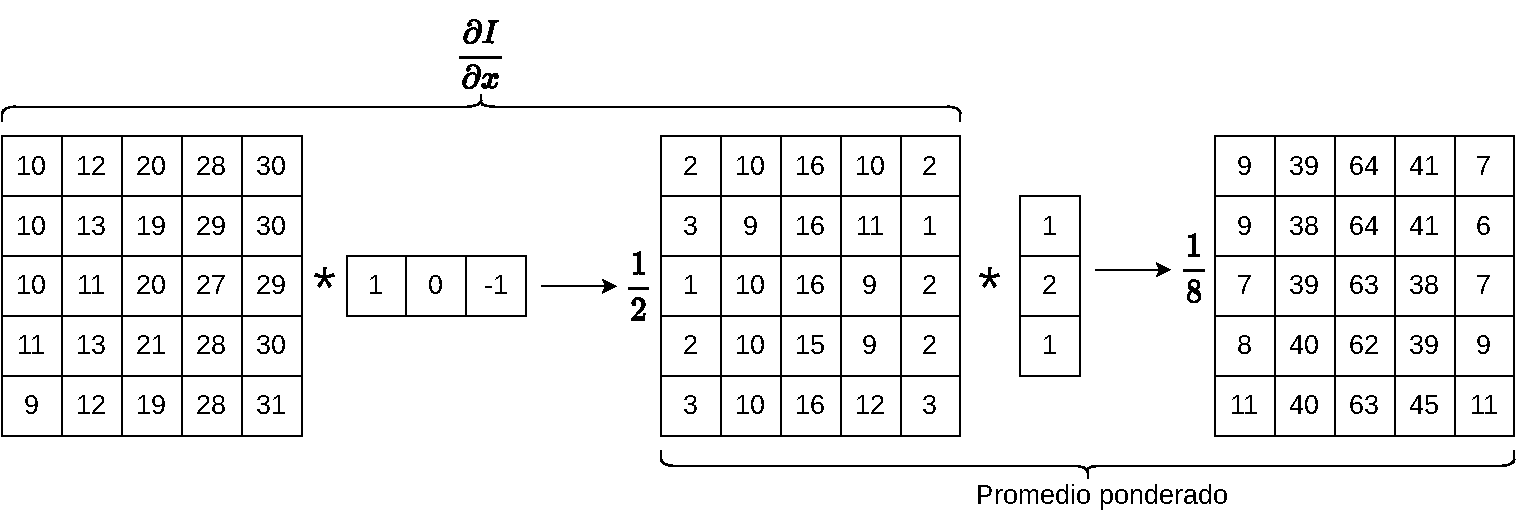
\includegraphics[width=\textwidth]{Figures/SobelX1.pdf}
  Se realiza un proceso similar para la derivada parcial en $Y$. Aplicando la propiedad asociativa de la convolución, se obtienen los siguientes ekernels:
  \[S_x = \left[\begin{tabular}{ccc}1 & 0 & -1\\2 & 0 & -2\\1 & 0 & -1 \end{tabular}\right]\qquad\qquad
  S_y = \left[\begin{tabular}{ccc}1 & 2 & 1\\0 & 0 & 0\\-1 & -2 & -1 \end{tabular}\right]\]
\end{frame}

\begin{frame}\frametitle{Ejemplo}
\end{frame}

\begin{frame}\frametitle{Magnitud y Ángulo}
  El gradiente en cada pixel de la imagen se puede calcular mediante la approximación de las derivadas parciales:
  \begin{eqnarray*}
    \frac{\partial I}{\partial x} &\approx& I * Sx = G_x\\
    \frac{\partial I}{\partial y} &\approx& I * Sy = G_y\\
  \end{eqnarray*}
  En la mayoría de las aplicaciones es más últil expresar el gradiente en forma polar:
  \[ \nabla I = G_m \angle G_a \]
  Donde la magnitud del gradiente y la fase, para cada pixel, se calculan como:
  \begin{eqnarray*}
    G_{m_{i,j}} &=& \sqrt{G_{x_{i,j}}^2 + G_{y_{i,j}}^2}\\
    G_{a_{i,j}} &=& \atantwo(G_{y_{i,j}}, G_{y_{i,j}})\\
  \end{eqnarray*}
\end{frame}

\begin{frame}\frametitle{Detector de Bordes de Canny}
  El detector de bordes de Canny es un detector basado en gradiente que consta de los siguientes pasos básicos:
  \begin{enumerate}
  \item Obtención del gradiente en magnitud y ángulo, mediante operadores de Sobel
  \item Supresión de puntos no máximos
  \item Aplicación de un doble umbral
  \end{enumerate}
  Aunque no es un paso en sí del Detector de Canny, generalmente se considera como primer paso la aplicación de un filtro Gaussiano para disminuir el ruido. 
\end{frame}

\begin{frame}\frametitle{Obtención del gradiente}
  Después del filtro Gaussiano, el primer paso es obtener el gradiente de la imagen mediante el Filtro de Sobel, en la forma de magnitud y ángulo:\\
  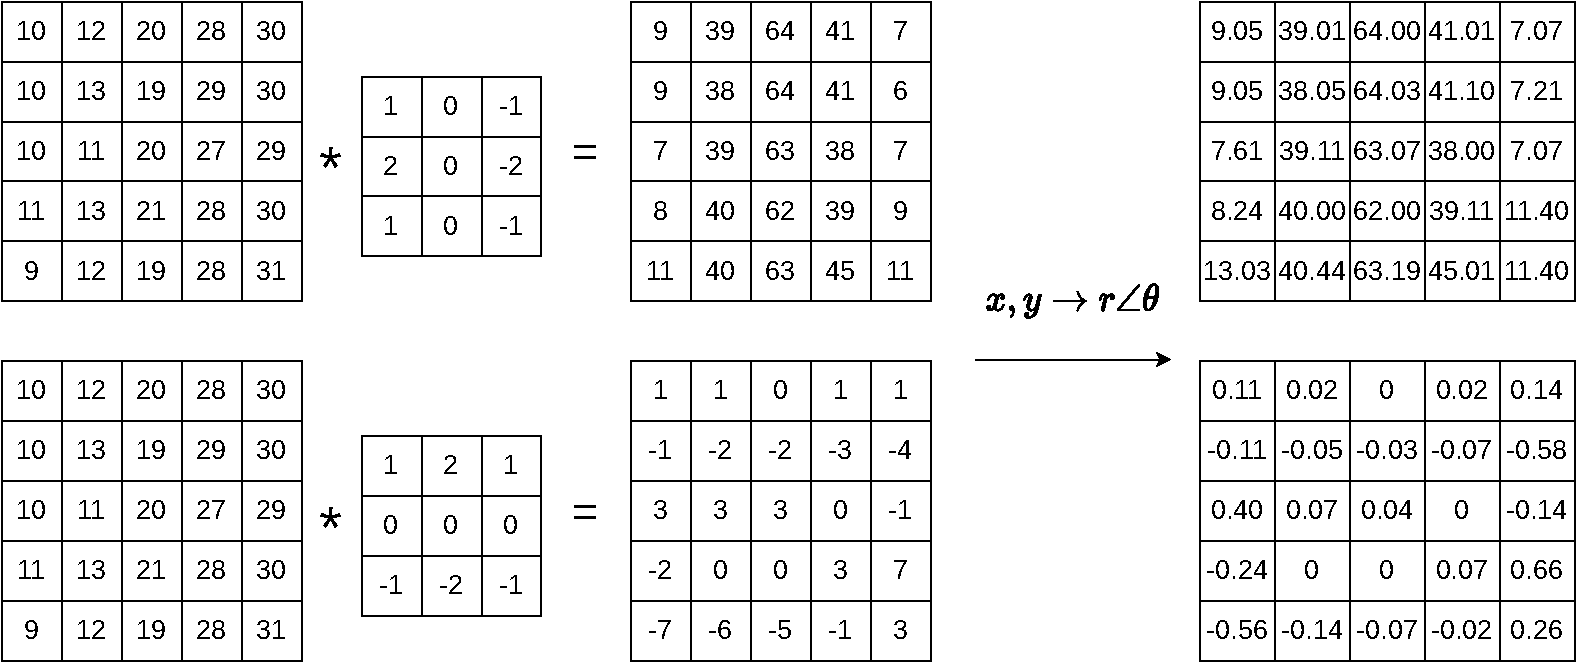
\includegraphics[width=0.9\textwidth]{Figures/SobelXY.pdf}
\end{frame}

\begin{frame}\frametitle{Supresión de no máximos}
  Este paso consiste en comparar la magnitud de cada pixel, con los pixeles anterior y posterior en la dirección del gradiente.
  Aunque la fase es un ángulo en $[-\pi, \pi]$, la dirección del gradiente se debe redondear a algún valor correspondiente a la connectividad 8: \textit{N, NE, E, SE}. Debido a que el pixel se compara en la dirección positiva y negativa del gradiente, no es necesario considerar las direcciones \textit{S, SW, W, NW}.
  \begin{figure}
    \centering
    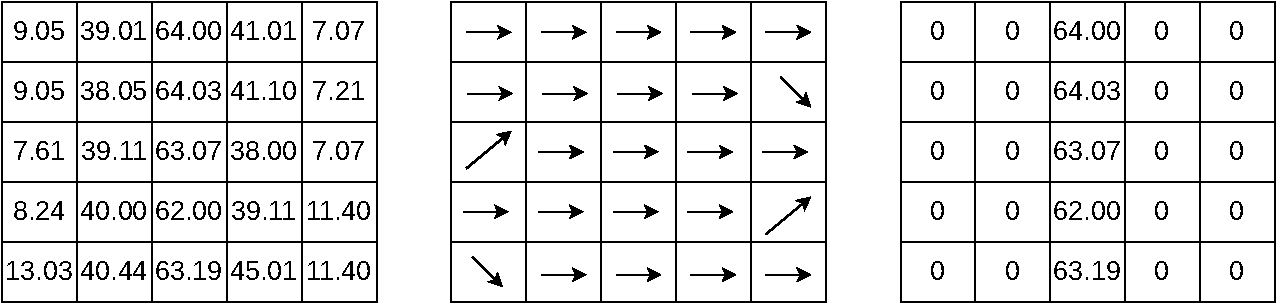
\includegraphics[width=0.9\textwidth]{Figures/SobelMA.pdf}
  \end{figure}
  Para cada pixel $p_i$, considere $p_{i+1}$, el pixel siguiente en la dirección del gradiente, y $p_{i-1}$, el pixel anterior, en la dirección del gradiente. El valor para cada pixel $q_i$ en la imagen resultante es:
  
  \[q_i = \begin{cases}p_i\qquad\qquad\textrm{si}\qquad p_i > p_{i+1} \qquad\textrm{y}\qquad p_i > p_{i-1}\\
  0\qquad\qquad\textrm{en otro caso}\end{cases}\]
\end{frame}

\begin{frame}\frametitle{Aplicación de doble umbral}
  En este paso, se definen dos umbrales: superior $\theta_u$ e inferior $\theta_l$. Los pixeles se clasifican en tres tipos:
  \begin{itemize}
  \item Fuertes: pixeles con magnitud del gradiente mayor que el umbral superior $|\nabla | > \theta_u$
  \item Débiles: pixeles con magnitud del gradiente entre ambos umbrales $\theta_l < |\nabla| < \theta_u$
  \item Suprimidos: pixeles con magnitud del gradiente menor que el umbral inferior $|\nabla| < \theta_l$
  \end{itemize}
  La imagen resultante se forma con las siguientes reglas:
  \begin{itemize}
  \item Todos los pixeles fuertes son parte de un borde.
  \item Todos los pixeles suprimidos no son bordes. 
  \item Los pixeles débiles son parte de un borde solo si están conectados (en conectividad 8) con un pixel fuerte.
  \end{itemize}
  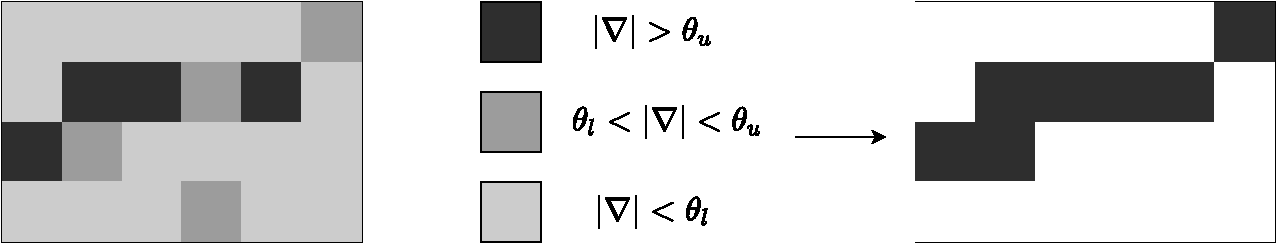
\includegraphics[width=\textwidth]{Figures/DoubleThreshold.pdf}
\end{frame}

\begin{frame}\frametitle{Espacios de color}
En las imágenes el color se representa mediante la combinación de 3 valores (generalmente, 3 bytes). Las diferentes formas de representar el color mediante estos tres valores se conocen como \textit{espacios de color}.
\end{frame}

\section{Características}

\begin{frame}\frametitle{Extracción de características}
  \begin{itemize}
  \item Las \textit{características} (\textit{features}) son conjuntos de valores derivados de una señal o de un conjunto de mediciones, que permiten describir el conjunto original y que son informativos y no redundantes.
  \item   Unas de las características más simples que se pueden extraer de una imagen son líneas y otras formas geométricas simples.
  \item El vector de características que describe una línea puede ser el conjunto de parámetros de su ecuación.
  \item Los vectores de características también se pueden utilizar para reconocer objetos, usando características cmo color, tamaño, forma, volumen, entre otras.
   \item Más adelante se verá la Transformada SIFT, uno de los algoritmos más usados para extracción de características. 
  \end{itemize}
\end{frame}

\begin{frame}\frametitle{La Transformada Hough}
  La Transformada Hough es un método que permite encontrar líneas, círculos y otras formas geométricas que se puedan describir fácilmente mediante expresiones analíticas. En el caso de las líneas, se trata de encontrar los dos parámetros que describen la recta:
  \begin{columns}
    \begin{column}{0.4\textwidth}
      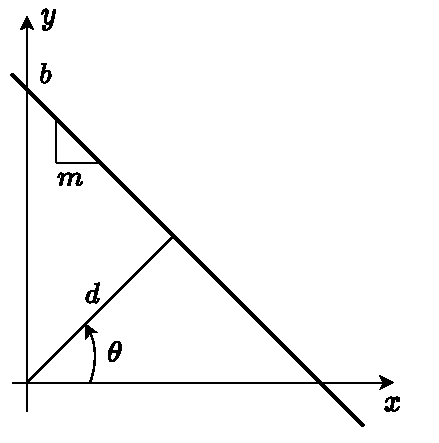
\includegraphics[width=\textwidth]{Figures/Hough2.pdf}
    \end{column}
    \begin{column}{0.6\textwidth}
      \begin{itemize}
      \item La forma pendiente-ordenada $y = mx + b$ tiene la desventaja de no poder expresar líneas verticales.
      \item La forma canónica $Ax + By + C$ requiere de una normalización $A_1 x + B_1 y + 1 = 0$ para que solo sean dos parámetros.
      \item Una forma más conveniente, es la forma normal $d = x\cos\theta + y\sin\theta$
      \item Esta última forma tiene una ventaja: si la línea correponde a un borde, el ángulo $\theta$ será la dirección del gradiente. 
      \end{itemize}
    \end{column}
  \end{columns}
\end{frame}

\begin{frame}\frametitle{El Espacio de Hough}
  El Espacio de Hough, para el caso de las líneas, es el conjunto de todos los posibles pares $(\theta, d)$.
  \begin{itemize}
  \item Una recta $L$ en el espacio cartesiano corresponde a un punto $P_h$ en el Espacio de Hough
  \item Un punto $P_c$ en el espacio cartesiano corresponde a una curva $C$ en el Espacio de Hough. Esta curva representa los parámetros $(\theta_i, d_i)$ de todas las rectas $L_i$ que pasan por el punto $P$.
  \end{itemize}
  \begin{figure}
    \centering
    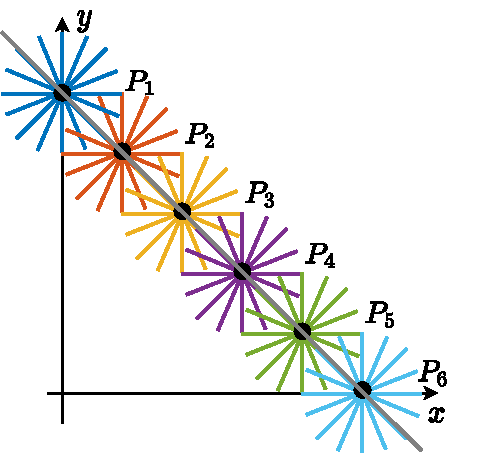
\includegraphics[width=0.35\textwidth]{Figures/Hough1.pdf}
    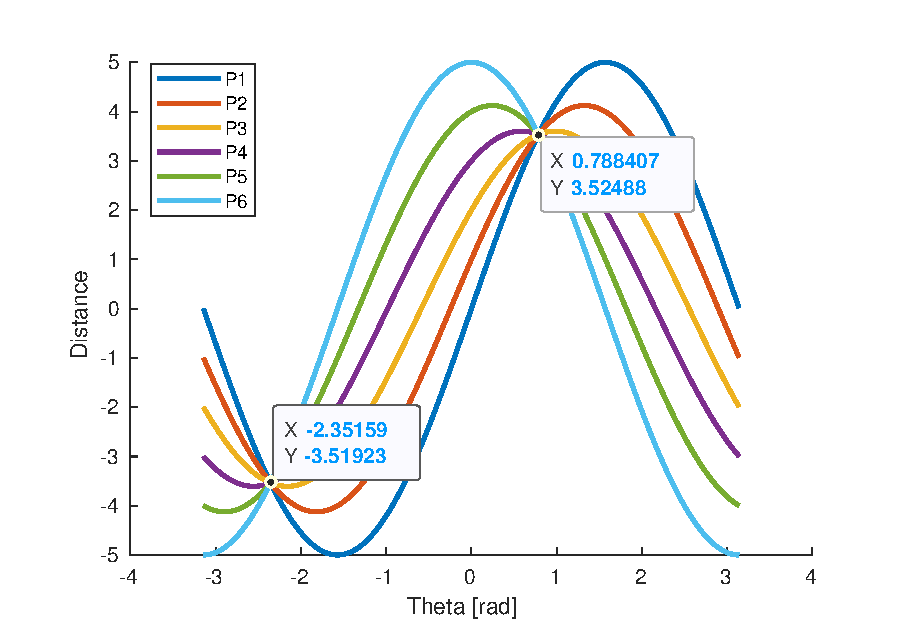
\includegraphics[width=0.5\textwidth]{Figures/Hough1.eps}
  \end{figure}
\end{frame}

\begin{frame}\frametitle{Extracción de Líneas por Transformada Hough}
  Este método consiste en encontrar las curvas $C_i$ en el espacio de Hough que pasan por cada punto $P_c$ en el espacio cartesiano. Los puntos $P_h$ en el Espacio de Hough por donde pasen más curvas $C_i$ corresponderán a las rectas resultantes en el espacio cartesiano.
  \begin{figure}
    \centering
    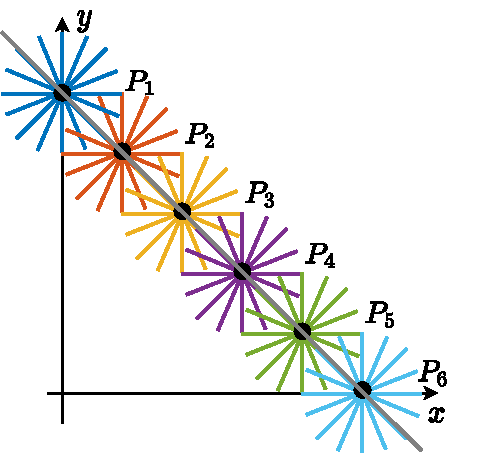
\includegraphics[width=0.35\textwidth]{Figures/Hough1.pdf}
    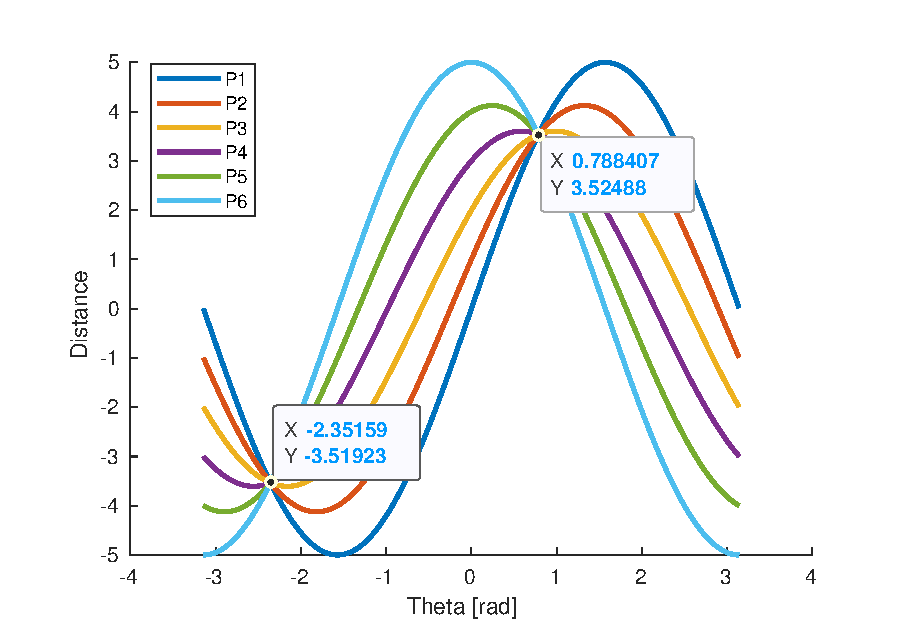
\includegraphics[width=0.5\textwidth]{Figures/Hough1.eps}
  \end{figure}
\end{frame}

\begin{frame}\frametitle{Extracción de Líneas por Transformada Hough}
  \begin{algorithm}[H]
    \KwIn{Imagen binaria $M$, umbral mínimo de votos $a_{min}$}
    \KwOut{Líneas expresadas en la forma $(d,\theta)$}
    \DontPrintSemicolon
    \;
    Inicializar en 0 un conjunto $A$ de acumuladores para cada par cuantizado $(d_k,\theta_k)$\;
    \ForAll{Pixel $M[i,j] \neq 0$}
    {
      \ForAll{Ángulo $\theta_k$ cuantizdo}
      {
        $d = j\cos\theta_k + i\sin\theta_k$
        $d_k = $ valor cuantizado de $d$
        Incrementar en uno el acumulador correspondiente $A[d_k, \theta_k]$
      }
    }
    \ForAll{$a \in A$}
    {
      \If{$a > a_{min}$}
      {
        Agregar la línea $(d_k, \theta_k)$ al conjunto de líneas detectadas
      }
    }
    Devolver el conjunto de líneas detectadas
  \end{algorithm}
\end{frame}

\begin{frame}\frametitle{Extracción de círculos por T. Hough}
  De la ecuación de un círculo en el plano:
  \[(x - c_x)^2 + (y - c_y)^2 = r^2\]
  Se puede observar que un círculo está definido por tres parámetros $(c_x, c_y, r)$.
  \begin{itemize}
  \item De forma similar a las líneas, se podrían fijar dos parámetros y calcular el tercero
  \item Sin embargo variar dos parámetros incrementa la complejidad considerablemente
  \item Se puede utilizar el ángulo del gradiente y un variar el valor del radio $r$ para determinar el centro, de este modo, solo se tiene que variar un parámetro.
  \item Se considera que el gradiente apunta hacia el centro del círculo. 
  \end{itemize}
\end{frame}

\begin{frame}\frametitle{T. Hough Generalizada}
  Hasta el momento la T. Hough se ha usado para detectar formas determinadas analíticamente. Se pueden detectar formas arbitrarias si se dispone de una descripción de la forma a detectar y, al igual que con círculos y líneas, se varían los parámetros y se hace un sistema de votos.
  \begin{itemize}
  \item La descripción de la forma se hace mediante la llamada \textit{Tabla R}
  \item Los parámetros que se pueden variar son el centro $(x_c, y_c)$, la rotación $\theta$ y la escala $(S_x, S_y)$
  \end{itemize}
  
\end{frame}

\begin{frame}\frametitle{T. H. Generalizada - Tabla R}
  La Tabla R es una descripción de la figura en función del ángulo del gradiente.
  \begin{figure}
    \centering
    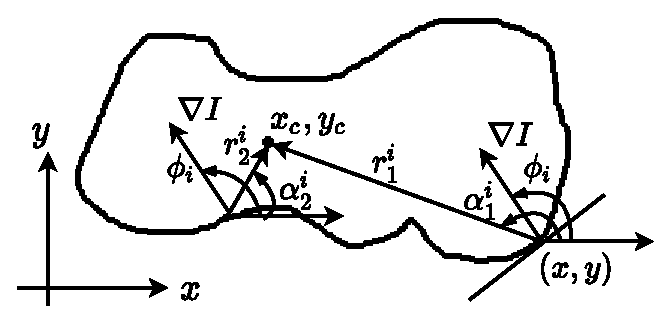
\includegraphics[width=0.5\textwidth]{Figures/HoughTableR.pdf}
  \end{figure}
  \begin{itemize}
  \item Se selecciona un centro arbitrario $(x_c, y_c)$
  \item Para cada punto $(x,y)$ en la figura, se calcula el ángulo del gradiente y se cuantiza a un ángulo $\phi_i$. 
  \item Para el mismo punto, se calcula el vector del punto al centro $(x_c - x, y_c - y)$ que se puede expresar en la forma polar $(r,\alpha)$
  \item A cada ángulo cuantizado $\phi_i$ se le pueden asociar varios valores $(r_1^i, \alpha_1^i),\dots , (r_j^i, \alpha_j^i)$
  \end{itemize}
\end{frame}

\begin{frame}\frametitle{T. H. Generalizada - Tabla R}
  Con la información anterior se construye la Tabla R:
  \[\]
  \begin{table}
    \centering
  \begin{tabular}{l|l}
    Ángulo del Gradiente & Vector al centro \\
    \hline
    $\phi_1$ & $(r_1^1, \alpha_1^1),\dots , (r_j^1, \alpha_j^1)$\\
    $\phi_2$ & $(r_1^2, \alpha_1^2),\dots , (r_j^2, \alpha_j^2)$\\
    $\vdots$ & $\vdots$\\
    $\phi_i$ & $(r_1^i, \alpha_1^i),\dots , (r_j^i, \alpha_j^i)$\\
    $\vdots$ & $\vdots$\\
    $\phi_n$ & $(r_1^n, \alpha_1^n),\dots , (r_j^n, \alpha_j^n)$
  \end{tabular}
  \end{table}
  \[\]
  La Tabla R funciona como una descripción de la forma arbitraria.
\end{frame}

\begin{frame}\frametitle{Detección de formas generales}
  El caso más sencillo se da cuando se tiene una forma en la imagen del mismo tamaño y orientación que el patrón original. En este caso solo es necesario determinar el centro, por lo que el Espacio de Hough solo tiene dos dimensiones: los parámetros $x_c, y_c$.
  \begin{algorithm}[H]
    \small
    \KwIn{Imagen binaria $M$, umbral mínimo de votos $a_{min}$}
    \KwOut{Formas generales definidas por la tabla R con centro en $(x_c,y_c)$}
    \DontPrintSemicolon
    \;
    Inicializar en 0 un conjunto $A$ de acumuladores para cada par cuantizado $(x_c,y_c)$\;
    \ForAll{Pixel $M[x,y] \neq 0$}
    {
      Determinar el ángulo $\phi$ del gradiente en el punto $x,y$ y cuantizarlo a un valor $\phi_i$\;
      \ForAll{Vector $(r_i^j, \alpha_i^j)$ asociado al ángulo $\phi_i$ en la Tabla R}
      {
        Determinar las coordenadas del centro:\;
        $x_c^j = x + \cos\alpha_i^j$\;
        $y_c^j = y + \sin\alpha_i^j$
        Incrementar en uno el acumulador correspondiente $A[x_c^j, y_c^j]$
      }
    }
    \ForAll{$a \in A$}
    {
      \If{$a > a_{min}$}
      {
        Agregar el patrón con centro en $(x_c, y_c)$ al conjunto de patrones detectados
      }
    }
    Devolver el conjunto de patrones detectados
  \end{algorithm}  
\end{frame}

\begin{frame}\frametitle{Detección de formas generales}
  Para detectar patrones con orientación $\theta$ y escala $S$ arbitrarios, se aplica el mismo principio, pero con un espacio de Hough de cuatro dimensiones: $(x_c, y_c, \theta, S$
  \begin{algorithm}[H]
    \small
    \KwIn{Imagen binaria $M$, umbral mínimo de votos $a_{min}$ }
    \KwOut{Formas generales definidas por la tabla $R$}
    \DontPrintSemicolon
    \;
    Inicializar en 0 un conjunto $A$ de acumuladores para cada tupla cuantizada $(x_c,y_c,\theta, S)$\;
    \ForAll{Pixel $M[x,y] \neq 0$}
    {
      Determinar el ángulo $\phi$ del gradiente en el punto $x,y$ y cuantizarlo a un valor $\phi_i$\;
      \ForAll{Orientación cuantizada $\theta$}
      {
        \ForAll{Escala cuantizada $S$}
        {
          \ForAll{Vector $(r_i^j, \alpha_i^j)$ asociado al ángulo $\phi_i$ en la Tabla R}
          {
            Determinar las coordenadas del centro:\;
            $x_c^j = x + S\cos(\alpha_i^j + \theta)$\;
            $y_c^j = y + S\sin(\alpha_i^j + \theta)$\;
            Incrementar en uno el acumulador correspondiente $A[x_c^j, y_c^j, \theta, S]$
          }
        }
      }
    }
    Devolver el conjunto de patrones donde el acumulador $A[x_c^j, y_c^j, \theta, S] > a_{min}$
  \end{algorithm}  
\end{frame}

\begin{frame}\frametitle{Detección de esquinas}
  Una esquina se puede considerar como un punto donde, en una vecindad $W$, el gradiente tiene dos direcciones dominantes diferentes.
  \begin{itemize}
  \item Aunque las esquinas representan un porcentaje muy pequeño de la imagen, suelen ser puntos de mucho interés.
  \item Las esquinas se consideran puntos de interés invariantes a escala, rotación e iluminación
  \item Entre algunas aplicaciones se encuentran:
    \begin{itemize}
    \item Registro de imágenes
    \item Reconstrucción de escenas 3D
    \item Detección de movimiento
    \item Reconocimiento de objetos
    \end{itemize}
  \end{itemize}
\end{frame}

\begin{frame}\frametitle{Detector de esquinas de Harris}
  Este detector se basa en la autocorrelación de los valores del gradiente en una vencidad de un pixel $(x,y)$. La detección se puede sintetizar en los siguientes pasos:
  \begin{itemize}
  \item Obtención de las derivadas parciales
  \item Obtención de la matriz del segundo momento
  \item Cálculo de la respuesta de Harris
  \item Supresión de no máximos
  \end{itemize}
\end{frame}

\begin{frame}\frametitle{Laplaciano de Gaussiano (LoG)}
  El Laplaciano de una función está definido como:
  \[\nabla^2 I = \frac{\partial^2 I}{\partial x^2} + \frac{\partial^2 I}{\partial y^2}\]
  Aplicando diferencias finitas, el Laplaciano se puede aproximar con el Kernel:
  \[\left[\begin{tabular}{ccc}0 & 1 & 0\\1 & -4 & 1\\0 & 1 & 0\end{tabular}\right]\]
\end{frame}

\bibliographystyle{abbrv}
\bibliography{References}
\end{document}
